Eines der Hauptthemen der Diplomarbeit ist die Überarbeitung des bisherigen Designs. 
Um dies zu erreichen, werden nicht nur über die aktuellen Standards und Trends analysiert, 
der aktuelle Content der Website restrukturiert und Usability-Tests durchgeführt, 
sondern auch ein mehrstündiger Workshop zum Thema UI/UX Design an der JKU absolviert.

\section{Recherche} \label{sec:Recherche}
\setauthor{Angerer Mona}
Um ein umfassendes Verständnis für die derzeit gängigen Designmethoden erhalten zu können, wurden zahlreiche bekannte große Websites wie die von Apple (....) und anderen analysiert.
Dabei werden die überschneidenden Merkmale identifiziert und herausgearbeitet und diejenigen, die für die HTL-Website besonders relevant sind, anschließend genauer untersucht. 
Auffällig ist dabei die übergeordnete Präferenz für das Motto „Weniger ist mehr“. Durchgehend dominiert minimalistisches Design mit vielen weißen Flächen, wodurch ein edler, strukturierter Eindruck erweckt wird.

Im Kontrast dazu werden jedoch auch viele Vektor- oder svg-Animationen, oftmals auch im „handgezeichneten“ Stil, verwendet, die das saubere Layout auflockern und Bewegung in die Benutzeroberfläche bringen. 

Darüber hinaus gewinnen Scrollingeffekte zunehmend an Bedeutung und werden von immer mehr Unternehmen als wichtiges und vielseitig einsetzbares Designelement betrachtet. 
Ob Parallax-Effekte, Scrollitelling, Immersive oder Horizontal Scrolling – das Weiterscrollen wird nicht mehr nur als „Bildschirminhalt verschieben“ gesehen, 
sondern wird zu einem immer wichtigeren, vielseitig eingesetzten Element. 

Ein weiterer interessanter Trend ist die verstärke Aufmerksamkeit auf individuell gestaltete
Error-Seiten. Diese werden zunehmend in das Gesamtdesign der Website integriert und mit kleinen 
Spielereien wie Animationen oder Mini-Games ausgeschmückt. 

Geometrische Ästhetik, insbesondere abstrakte Formen wie Dreiecke, 
Kreise, Vierecke oder eine Kombination davon, gewinnen im Web-Bereich deutlich sichtbar an Popularität. 
Auf vielen hochwertigen Websites tragen diese geometrischen Gestaltungselemente dazu bei, eine strukturierte und interessante Oberfläche zu schaffen. 


\section{Content-Strukturierung}
\setauthor{Angerer Mona}
Durch Gespräche mit SchülerInnen, Lehrkräften und InteressentInnen stellt sich hinaus, dass einer der am häufigsten bemängelten Aspekte der bisherigen 
HTL-Website der unübersichtliche Aufbau mit etlichen Unterseiten ist. Es fällt den Usern teilweise schwer, sich auf der Benutzeroberfläche zu orientieren 
und den gesuchten Inhalt auf Anhieb zu finden. Um dieses Problem zu beheben, wird zunächst eine eingehende Analyse des Menüs und seiner Unterpunkte durchgeführt, 
um einen umfassenden Überblick über den gesamten Website-Inhalt zu erhalten. Nach intensiver Prüfung wird anschließend festgestellt, dass durch eine Neustrukturierung von 
7 Menüpunkten auf nur noch 5 Hauptseiten übergegangen werden kann.

Des Weiteren wird ein erheblicher Teil des Inhalts von der Website ins LeoWiki, das interne Wiki der HTL Leonding, ausgelagert. 
Dies verhindert, dass Content, der nur für Personen, die bereits an der HTL Leonding lernen oder lehren, relevant ist, für Außenstehende sichtbar ist und ermöglicht, 
dass die meisten Seiten keine weiteren Unterseiten besitzen und somit als One Pager fungieren, auf denen der Inhalt durch einfaches Scrollen zugänglich ist.



\section{Workshop}
\setauthor{Angerer Mona}
An dem Workshop auf dem Campus der JKU, der von … von der Firma KBC abgehalten wurde, nahmen beiden Diplomarbeitsteams, der Betreuungslehrer Herr Professor Huemer und die beiden Professorinnen 
Frau Engleitner und Frau Rammelmüller teil. 

Um einen Ausgangspunkt für die Entwicklung eines Designkonzepts zu schaffen, 
führt man zunächst eine umfassende Problemanalyse durch (Siehe Abbildung \ref{fig:impl:problemanalyse}). In Teams wird die bewährte Post-It-Methode angewendet, 
bei der jeder/jede TeilnehmerIn unterschiedlich farbige Zettel erhält, um Mängel und Verbesserungsvorschläge auf gemeinsame Plakate zu kleben. 
Dieser kollaborative Ansatz ermöglicht die Erstellung einer Art Mindmap, auf der die Schwächen der aktuellen HTL-Website deutlich herausgearbeitet werden. 
Dabei werden Herausforderungen wie die Unübersichtlichkeit des Menüs, eine zu bunte Gestaltung und Probleme im Mobile-Modus hervorgehoben. 
Diese Methode lenkt den Fokus von Anfang an auf die Lösungsfindung in Beachtung der bereits existierenden Probleme, um somit nicht nur eine Neuimplementierung, 
sondern eine konkrete Verbesserung der Website zu erreichen.

\begin{figure}
    \begin{minipage}[b]{.4\linewidth} 
       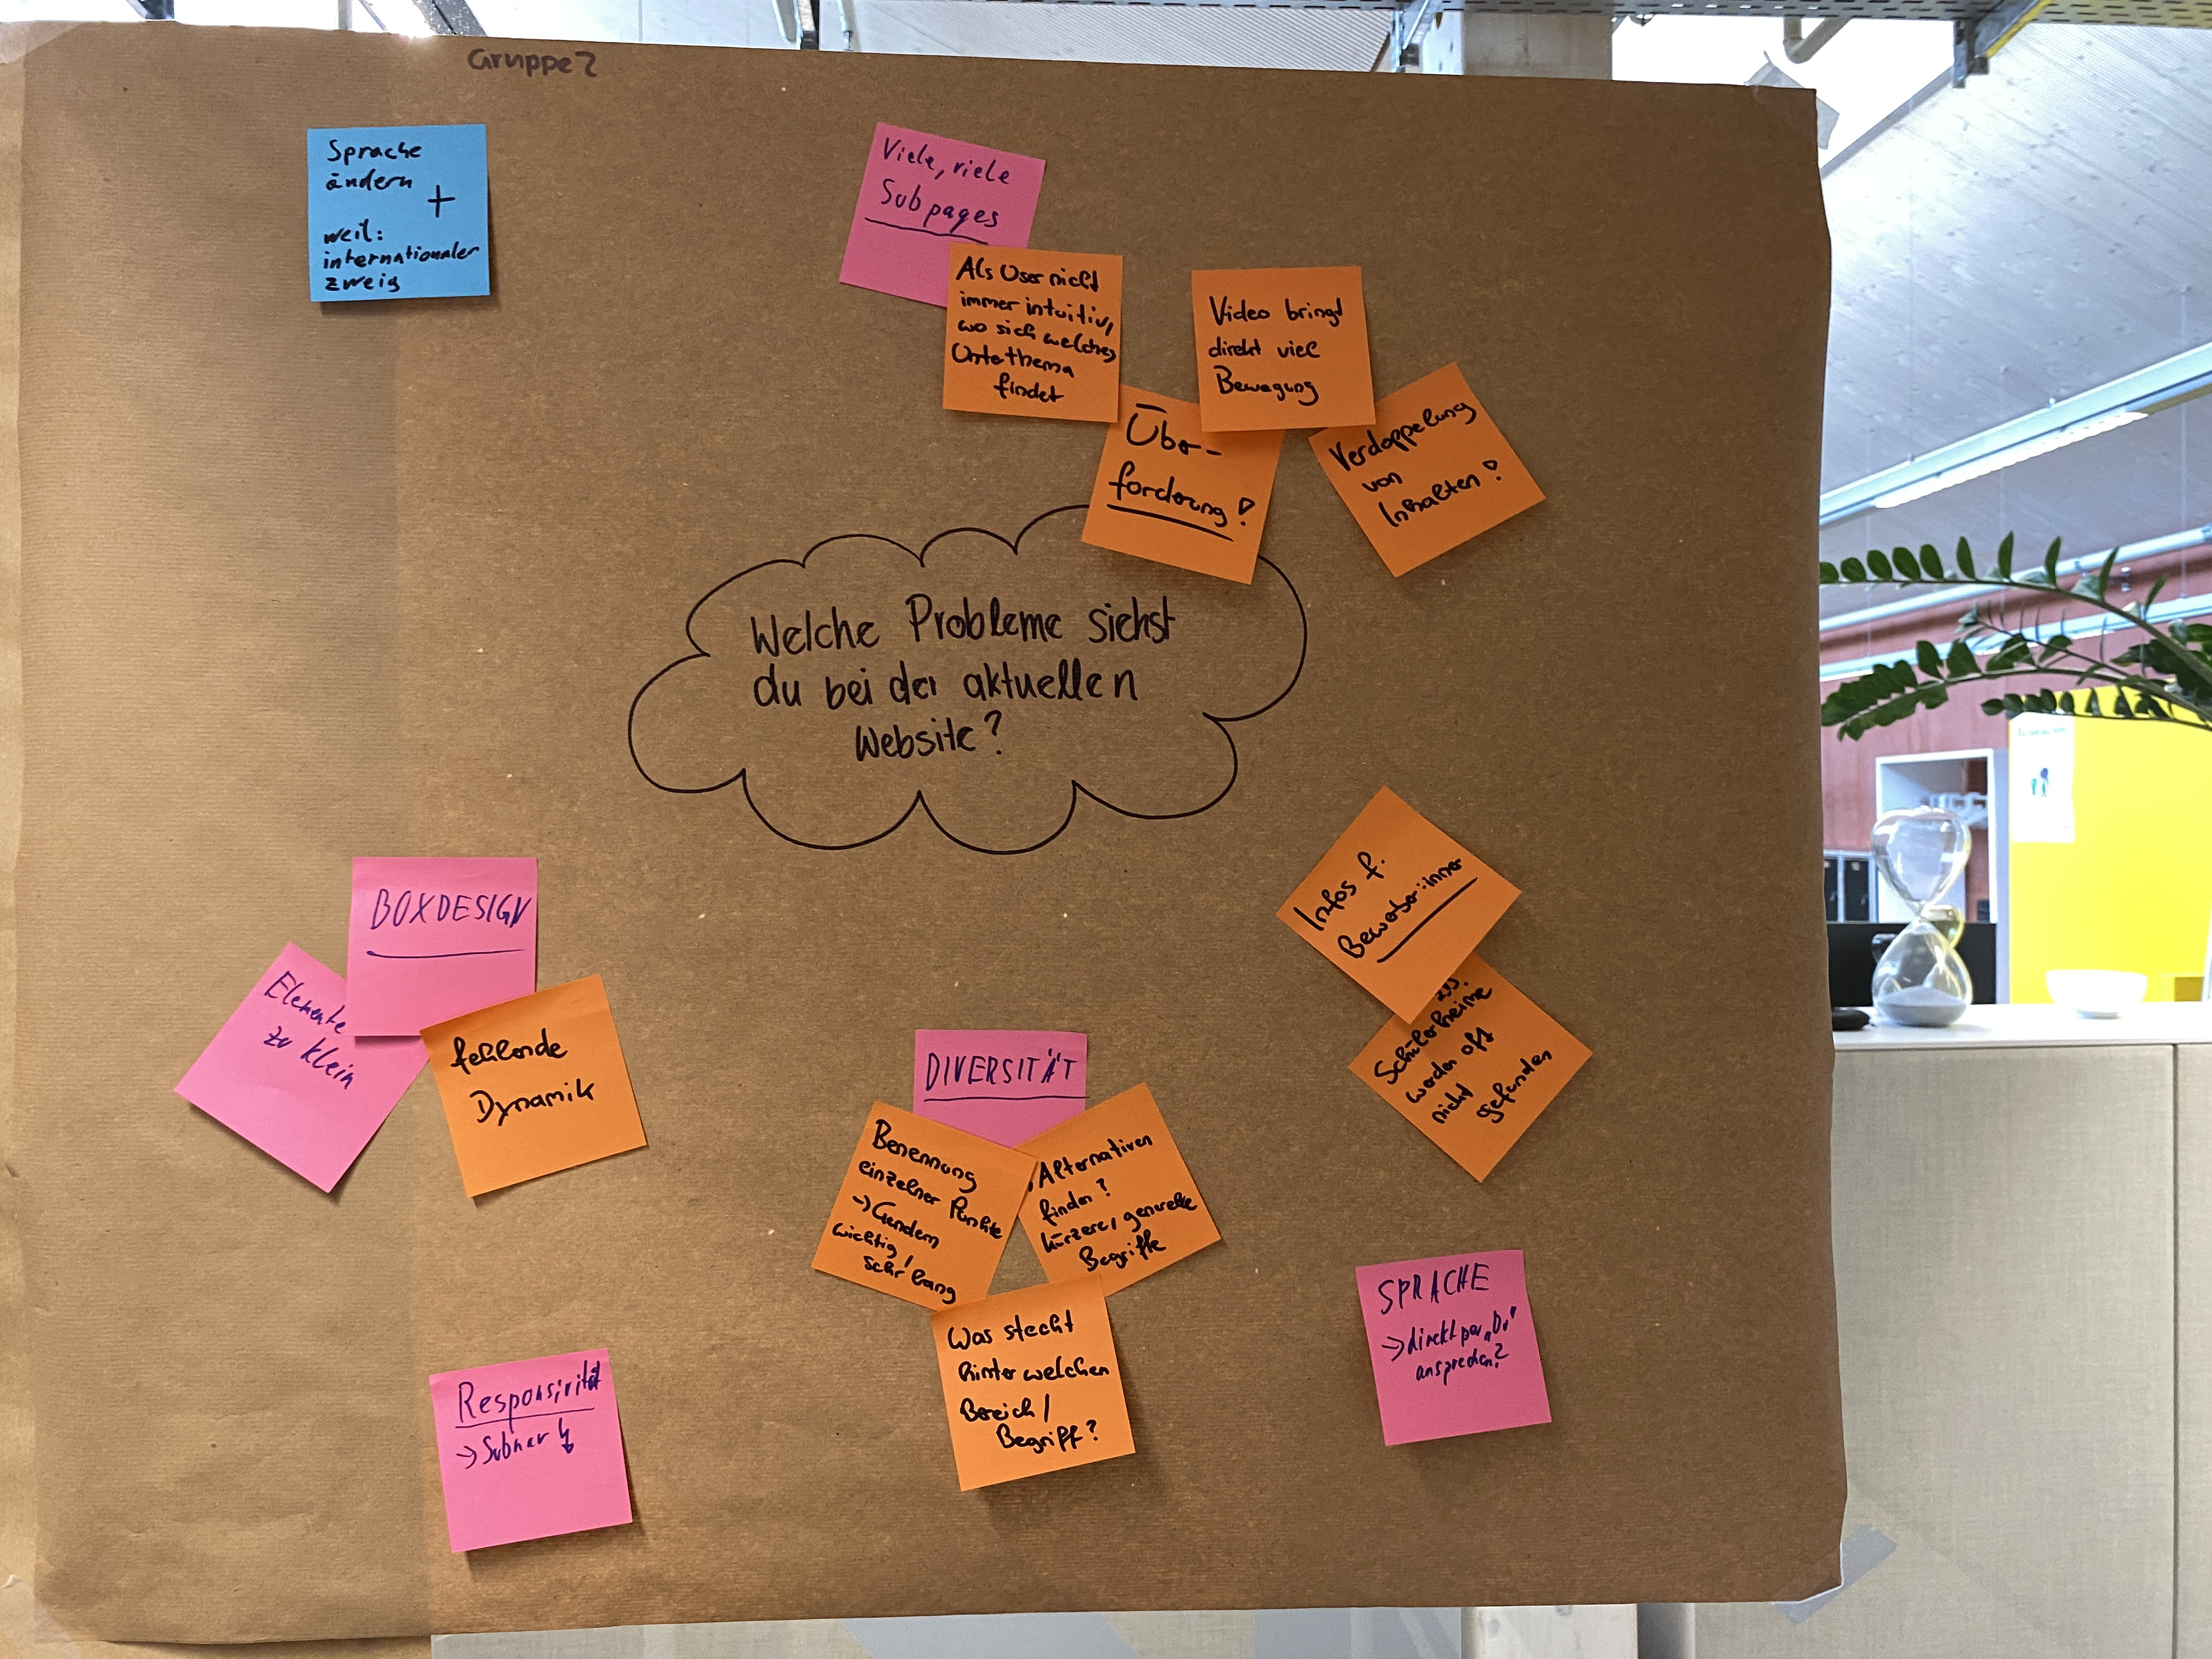
\includegraphics[width=\linewidth]{pics/problemanalyse.jpg}
       \caption{Problemanalyse}
       \label{fig:impl:problemanalyse}
    \end{minipage}
    \hspace{.05\linewidth}
    \begin{minipage}[b]{.4\linewidth}
       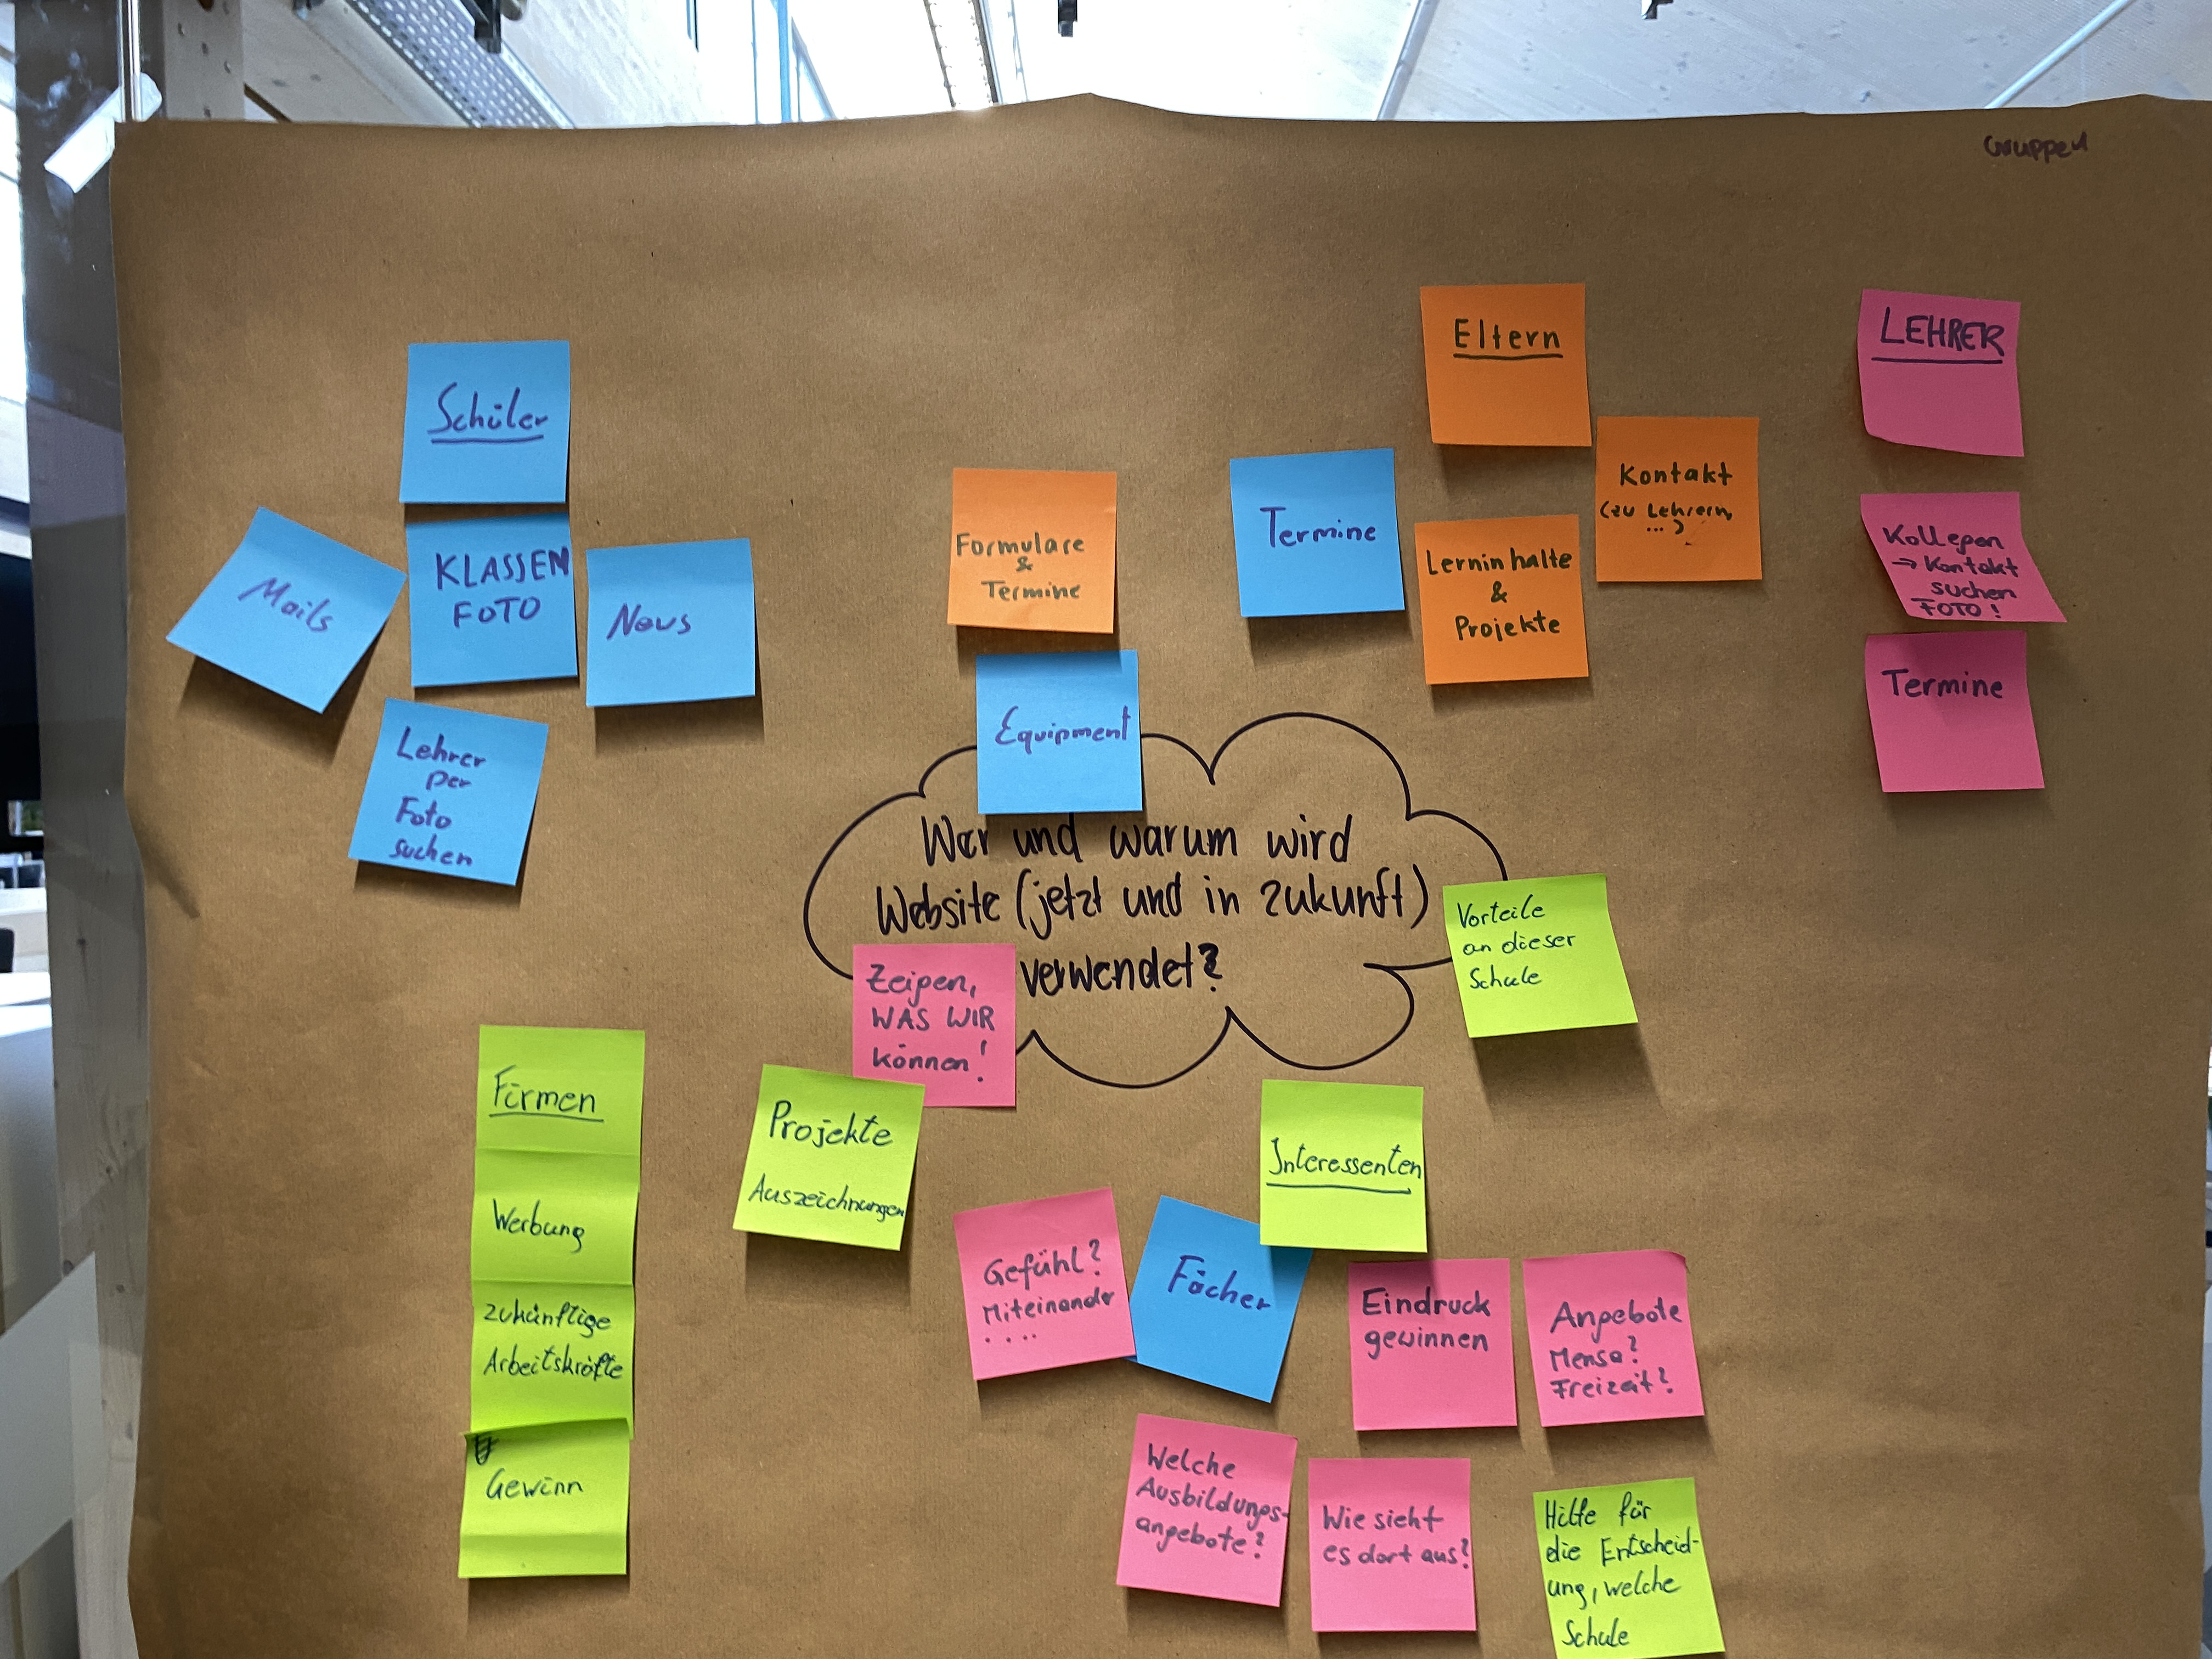
\includegraphics[width=\linewidth]{pics/zielgruppenanalyse.jpg}
       \caption{Zielgruppenanalyse}
       \label{fig:impl:zielgruppenanalyse}
    \end{minipage}
 \end{figure}

Der kreative kollaborative Prozess setzt sich fort und mündet in einer detaillierten Zielgruppenanalyse (Siehe Abbildung \ref{fig:impl:zielgruppenanalyse}). 
Dieser Schritt ist von besonderer Bedeutung in der Designentwicklung, da eine Benutzeroberfläche erst dann als gelungen betrachtet werden kann, 
wenn sie von den BenutzerInnen intuitiv genutzt werden kann und ihren individuellen Anforderungen gerecht wird. 
Bei der HTL-Website werden verschiedene Benutzergruppen identifiziert, darunter SchülerInnen, LehrerInnen, InteressentInnen, Firmen und Eltern. 
Zusätzlich berücksichtigt man deren spezifische Intentionen. Beispielsweise ist für Unternehmen von großem Interesse, 
welche Projekte an der Schule verfolgt werden und welche Technologien dafür verwendet werden. 
Eltern und InteressentInnen wiederum möchten vorrangig Informationen zu den angebotenen Zweigen und Fächern an der HTL erhalten, 
während Lehrkräfte und SchülerInnen insbesondere anstehende Events und Aktivitäten im Blick haben möchten. 
Diese präzise Zielgruppenanalyse bildet die Grundlage für ein benutzerzentriertes Designkonzept, das den Bedürfnissen aller Zielgruppen gerecht wird.


Um die Benutzerperspektive noch intensiver zu erfassen, geht man im weiteren Verlauf darauf ein, 
welche Gedanken, Wünsche, Handlungen und Emotionen die NutzerInnen während der Verwendung der Website durchlaufen (Siehe Abbildung \ref{fig:impl:user_gefühle}). 
Dabei werden nicht nur positive Gefühle und Gedanken, wie Vorfreude und Neugierde, herausgearbeitet, sondern auch potenzielle Ängste oder Unsicherheiten. 
Hierzu gehören beispielsweise Fragen wie: \glqq Bin ich gut genug für die HTL?\grqq oder \grqq Habe ich überhaupt Chancen, aufgenommen zu werden?\grqq.

Die Berücksichtigung dieser vielschichtigen Nutzererfahrungen ermöglicht eine empathische Gestaltung der Benutzeroberfläche, 
die nicht nur informativ ist, sondern auch dazu beiträgt, positive Emotionen zu fördern und mögliche Ängste zu mildern. 
Durch diese eingehende Analyse der Nutzerperspektive wird die HTL-Website nicht nur funktional, sondern auch emotional ansprechend und unterstützend gestaltet.

\begin{figure}
   \begin{minipage}[b]{.4\linewidth} 
      \includegraphics[width=\linewidth]{pics/user_gefühle_gedanken.JPG}
      \caption{UserInnen Gefühle}
      \label{fig:impl:user_gefühle}
   \end{minipage}
   \hspace{.05\linewidth}
   \begin{minipage}[b]{.4\linewidth}
      \includegraphics[width=\linewidth]{pics/user_missionen.JPG}
      \caption{UserInnen Missionen}
      \label{fig:impl:user:missionen}
   \end{minipage}
\end{figure}

Um eine intuitive Benutzererfahrung auf der Website sicherzustellen, werden darüber hinaus potenzielle Missionen, 
Gedankengänge und Vorgehensweisen der NutzerInnen berücksichtigt, die sie bei ihrem Besuch auf dem HTL-Webauftritt haben könnten (Siehe Abbildung \ref{fig:impl:user:missionen}). 
Es wurde dabei analysiert, welche konkreten Ziele sie verfolgen, welche Informationen sie suchen und welche Schritte sie wahrscheinlich unternehmen möchten.

Diese detaillierte Betrachtung der Nutzerinteraktion ermöglicht es, die Benutzeroberfläche so zu gestalten, dass sie den natürlichen Denk- und Handlungsmustern 
der BenutzerInnen entspricht. Durch das Verstehen der potenziellen Missionen und Gedankengänge wird sichergestellt, dass die Website nicht nur informativ ist, 
sondern auch nahtlos in den individuellen Ablauf der NutzerInnen integriert wird. Dieser Ansatz fördert eine reibungslose und effektive Nutzung der Website.

Mit dem erlangten Wissen über die zu behebenden Probleme und die unterschiedlichen Usergruppen, deren individuelle Anforderungen 
an die HTL-Website, die Ziele, die sie mit dem Besuch der Website verfolgen möchten und die Emotionen und Eindrücke, die man in den Usern beim benutzen der Oberfläche erwecken will,
wird nun der Startpunkt für die Erstellung eines Designentwurfs erleichtert. Dazu wurde unter den
TeilnehmerInnen des Workshops Zettel und Stifte ausgeteilt, um Skizzen und mögliche Layouts für die Weboberfläche zu gestalten. (Siehe Abbildung \ref{fig:impl:erste_entwuerfe})
Durch diese Methode werden eine Vielzahl an Ideen erbracht, die in der gesamten Gruppe geteilt und diskutiert werden. 
Dieser kreative Ansatz ermöglicht es, die gewonnenen Erkenntnisse 
unmittelbar in konkrete visuelle Konzepte umzusetzen und so den Grundstein für eine optimierte HTL-Website zu legen.

\begin{figure}
   \centering
   \begin{subfigure}{0.3\textwidth}
     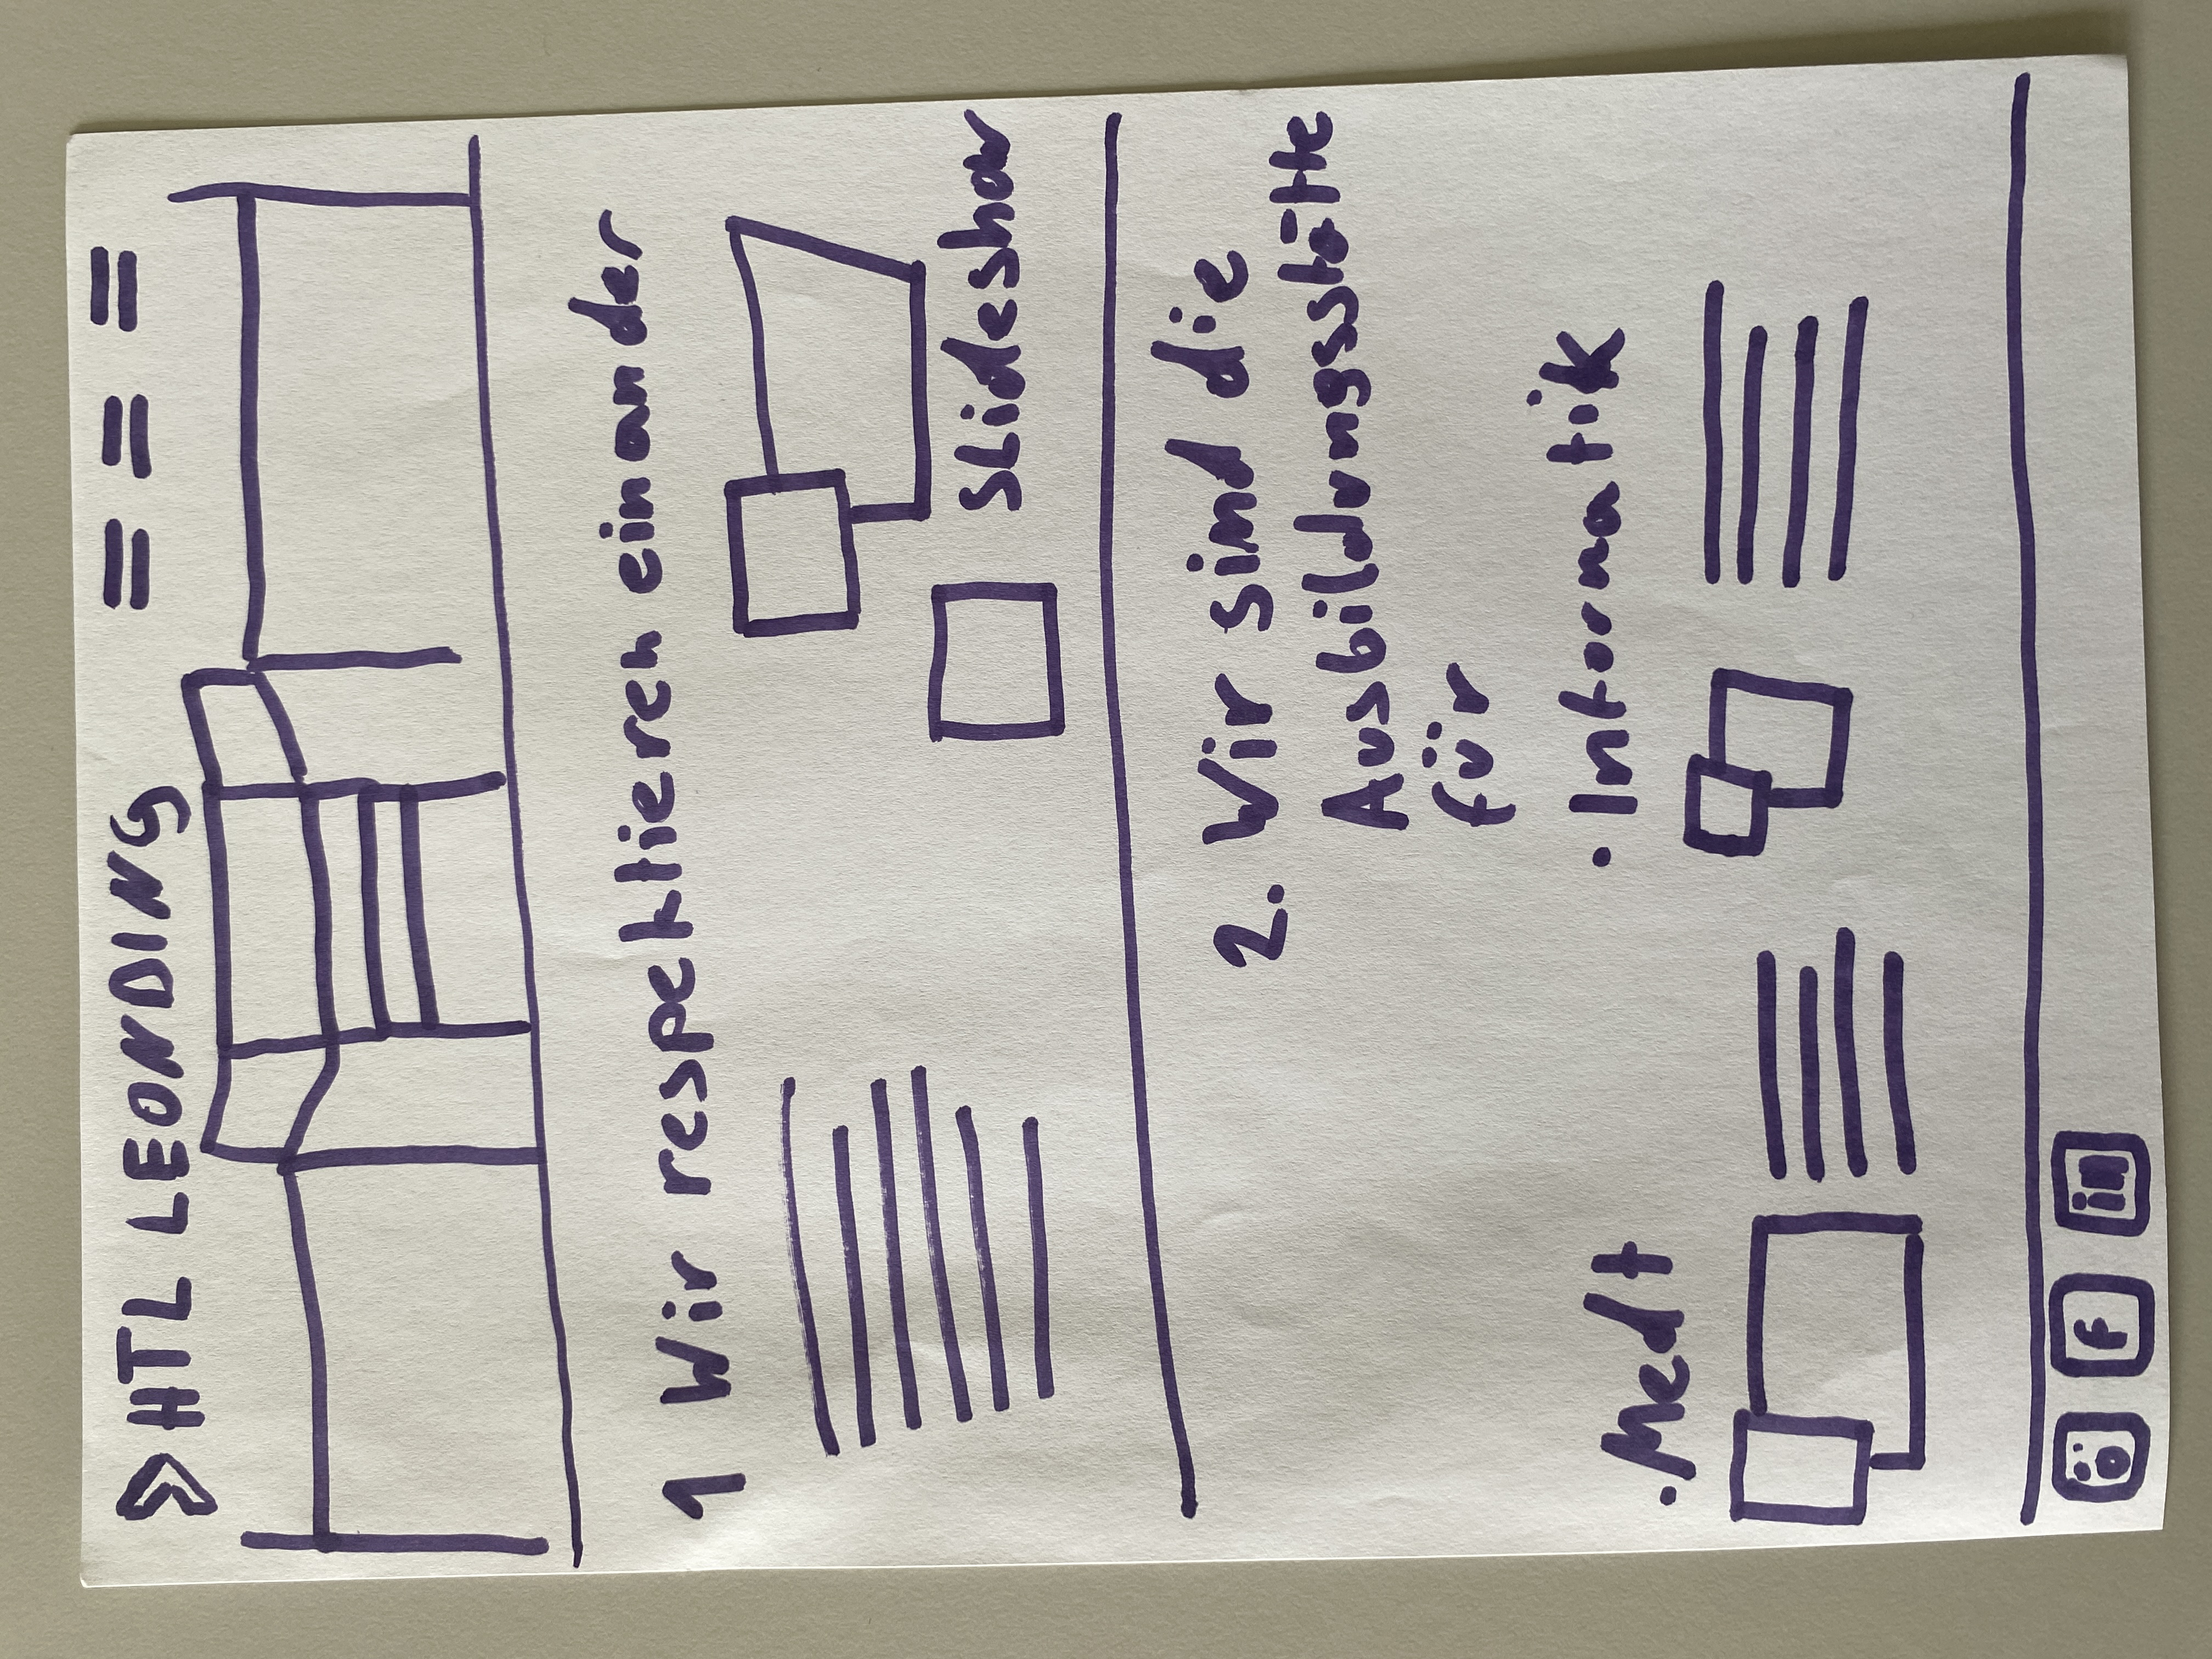
\includegraphics[width=\textwidth, angle=270]{pics/Entwurf_Beispiel_1.JPG}
     \caption{Entwurf 1}
     \label{fig:a}
   \end{subfigure}
   \hfill
   \begin{subfigure}{0.3\textwidth}
     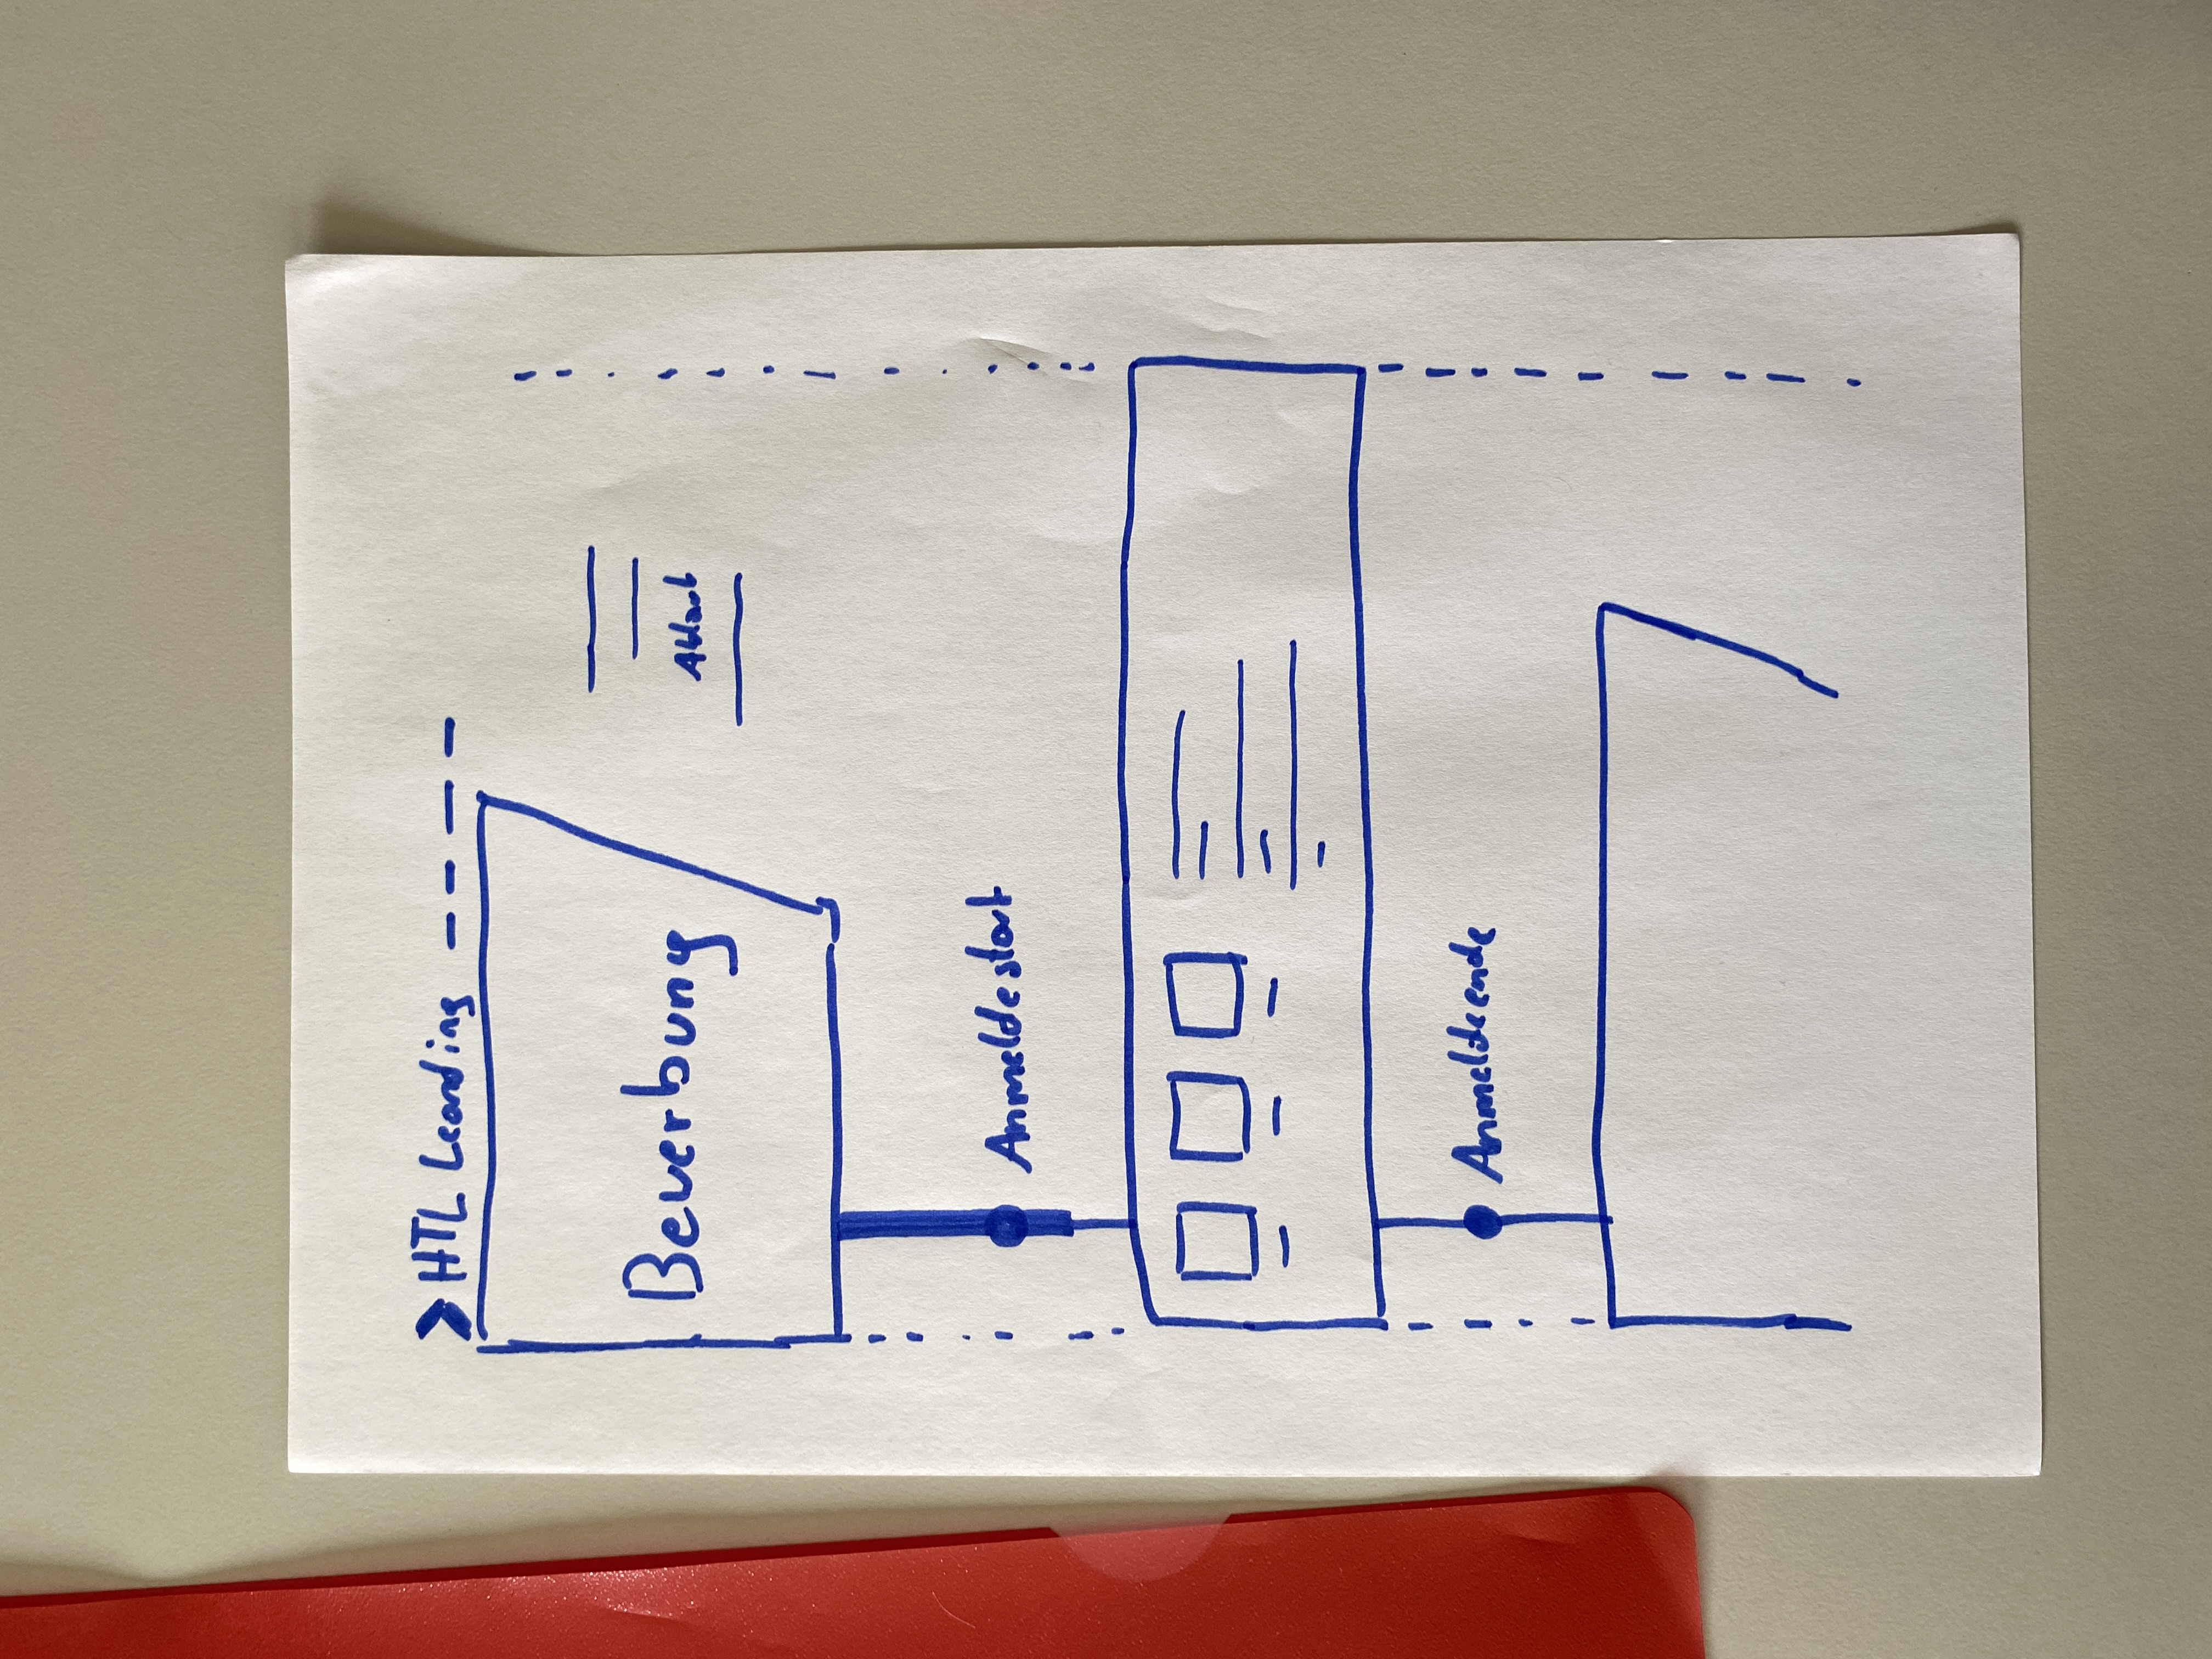
\includegraphics[width=\textwidth, angle=270]{pics/Entwurf_Beispiel_2.JPG}
     \caption{Entwurf 2}
     \label{fig:b}
   \end{subfigure}
   \hfill
   \begin{subfigure}{0.3\textwidth}
     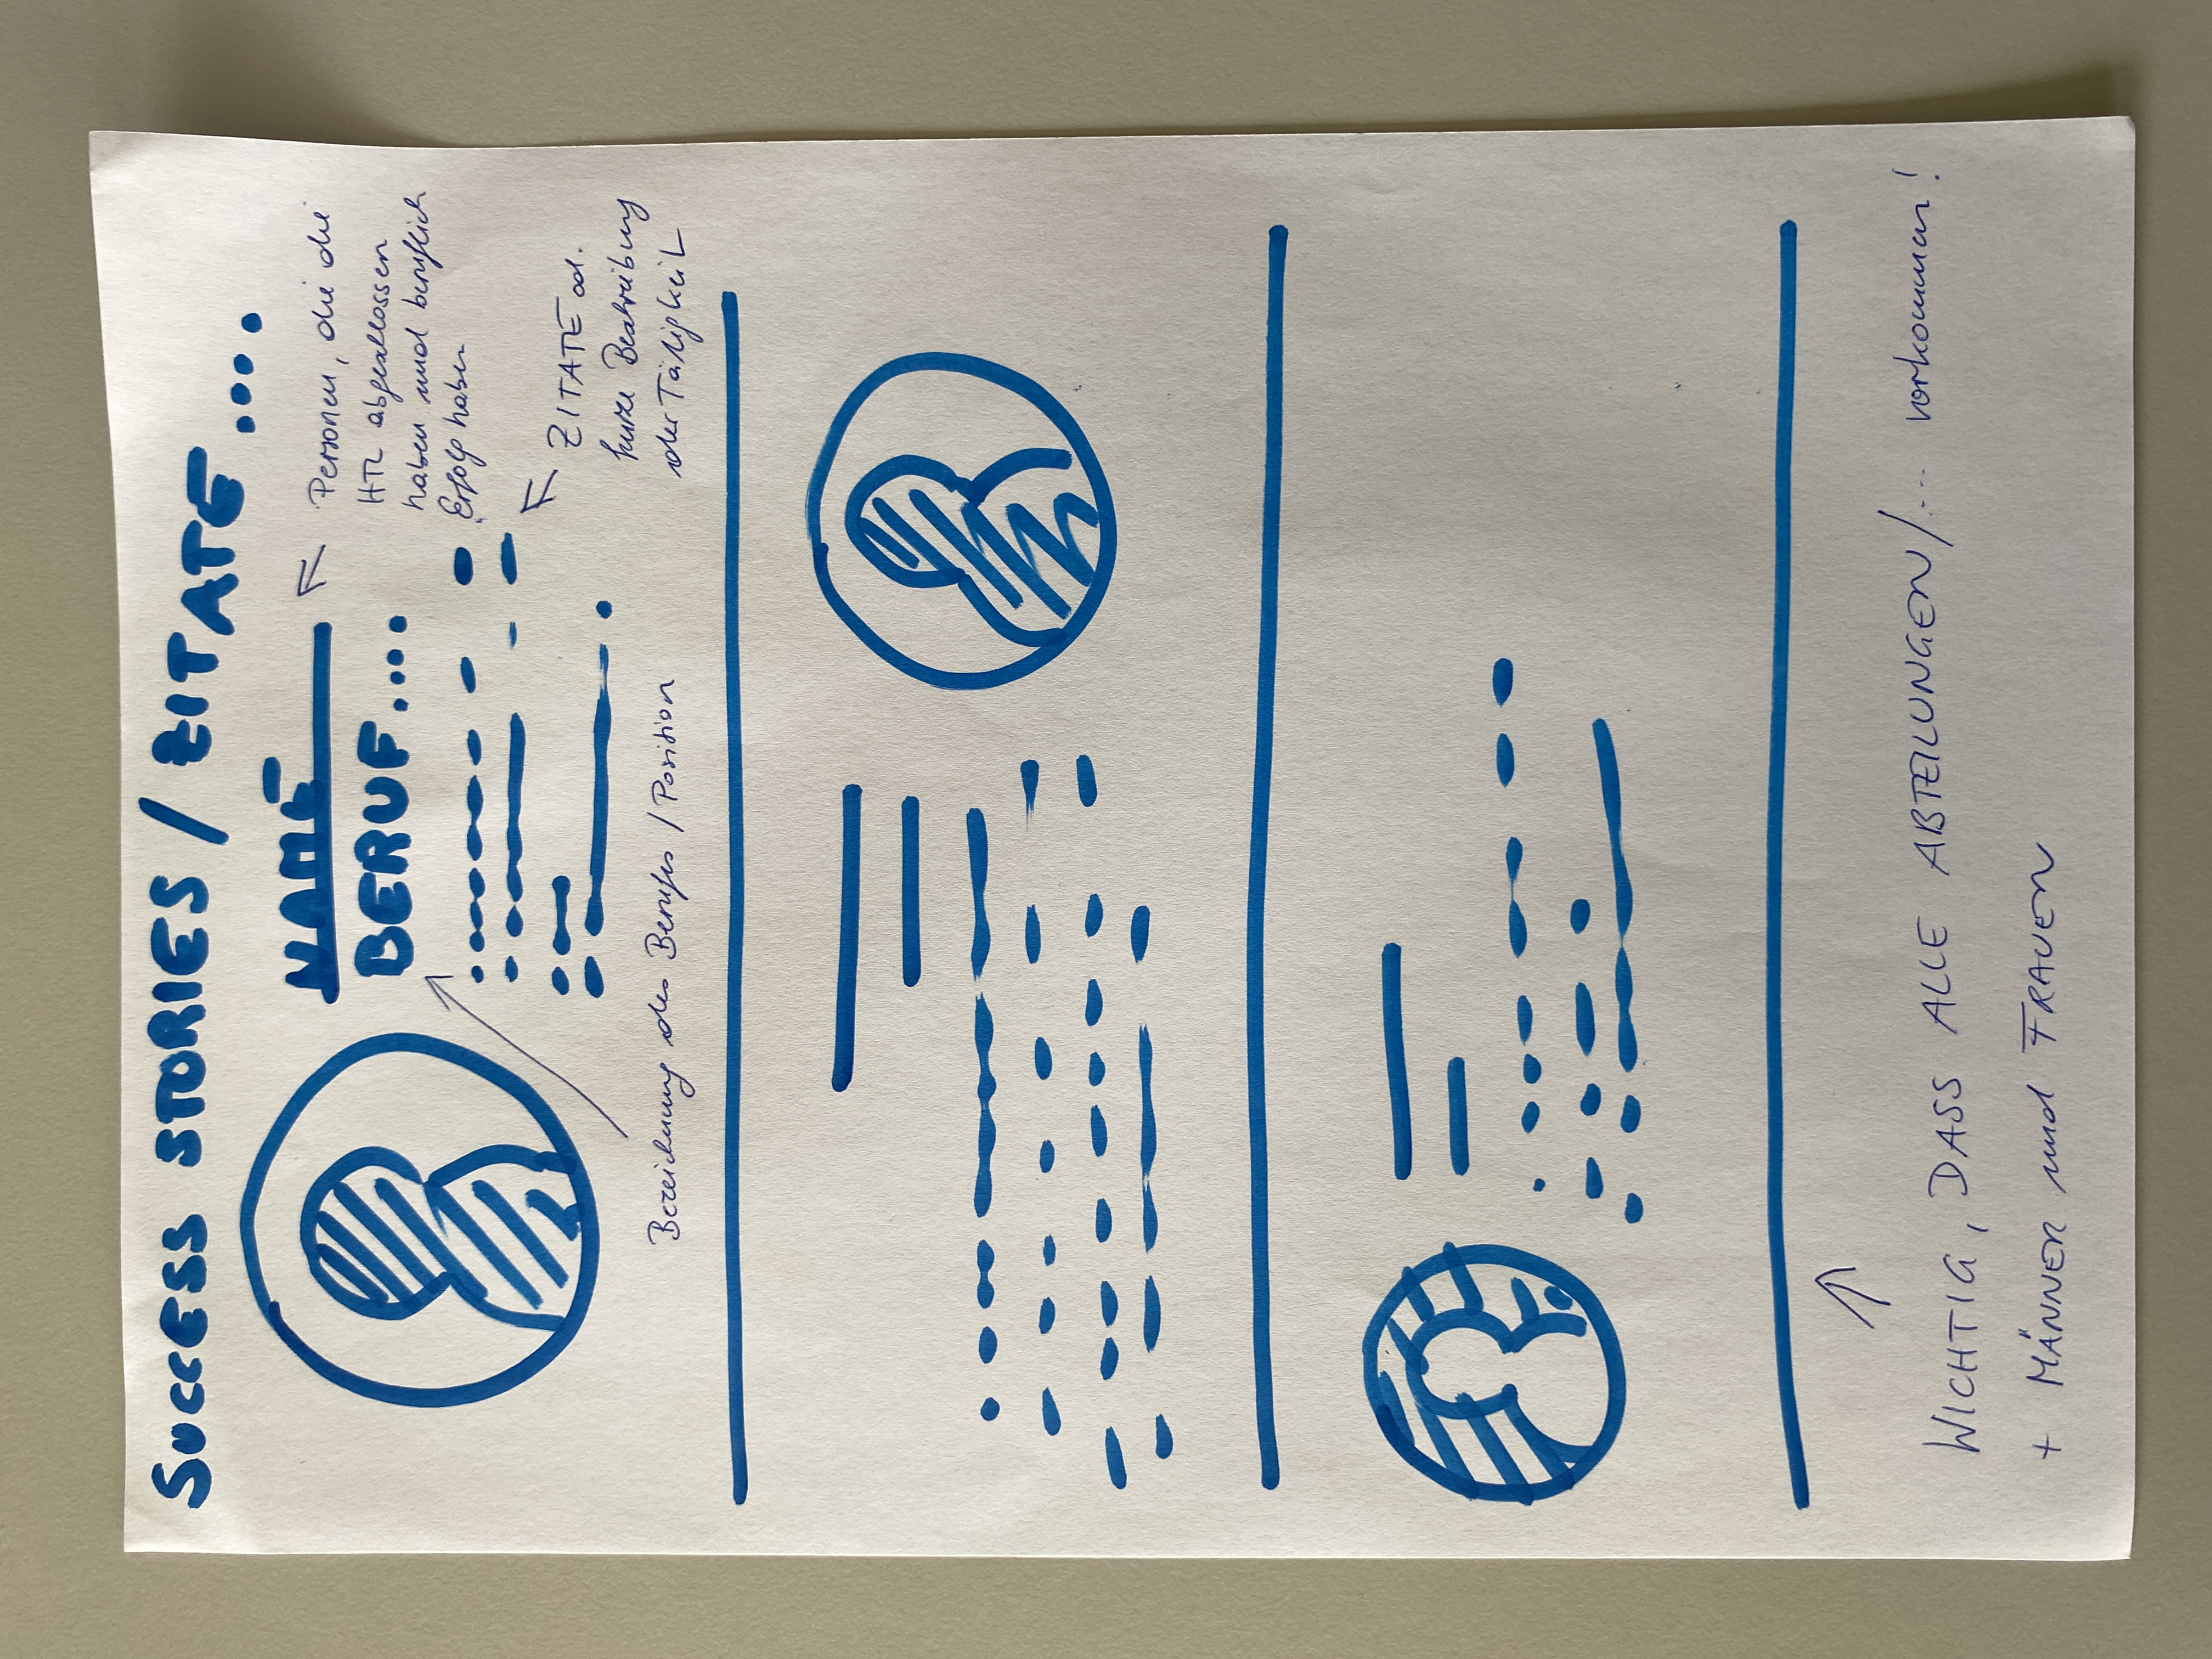
\includegraphics[width=\textwidth, angle=270]{pics/Entwurf_Beispiel_3.JPG}
     \caption{Entwurf 3}
     \label{fig:c}
   \end{subfigure}
   \caption{erste Entwürfe}
   \label{fig:impl:erste_entwuerfe}
 \end{figure}

\section{Entwurf und Usability-Tests}
\setauthor{Angerer Mona}
Nach umfassenden Analysen und Untersuchungen der geeigneten Gestaltungselemente, Effekte und Animationen für die HTL-Website wird unter Anwendung des im Workshop 
erworbenen Wissens und der Designmethoden ein erster Entwurf erstellt. Die Gestaltung wird mithilfe der Plattform Figma in Form eines 
Click-Dummies skizziert. (Siehe Abbildung \ref{fig:impl:figma_entwurf}) Anschließend präsentiert man diesen Entwurf SchülerInnen der ersten und zweiten Klasse der HTL sowie Lehrkräften 
und externen Personen. Diese Form der Testung ermöglicht es, direktes Feedback und Bewertungen zu sammeln, um den Entwurf 
weiter zu verfeinern und optimal an die Bedürfnisse der BenutzerInnen anzupassen. Der Prozess integriert somit gezielt die Perspektiven 
der verschiedenen Zielgruppen, um eine benutzerfreundliche Website zu gewährleisten. 
Die erhaltenen Rückmeldungen bekräftigen die verbesserte Struktur und die aufgewertete Anordnung durch die Reduzierung der Menüpunkte. 
Zudem wird bestätigt, dass die Navigation auf der Benutzeroberfläche merklich vereinfacht wurde. Allerdings werden auch einige Anregungen 
und Kritiken geäußert, darunter die Empfehlung, vermehrt Schülerfotos einzubinden, um die Website persönlicher zu gestalten. Diese Maßnahme 
soll dazu beitragen, ein einladenderes Bild der HTL Leonding zu vermitteln. Auch werden einige Verschiebungen von Inhalt in andere Menüpunkte 
vorgeschlagen, um eine logischere Anordnung sicherzustellen. 
Nach der Implementierung dieser Verbesserungsvorschläge wird der Prozess mehrfach wiederholt, um das Design weiter zu perfektionieren und 
eine optimale Zufriedenheit aller BenutzerInnen sowie eine intuitive Steuerung der Website zu erreichen. 

\begin{figure}
   \begin{minipage}[b]{\linewidth} 
      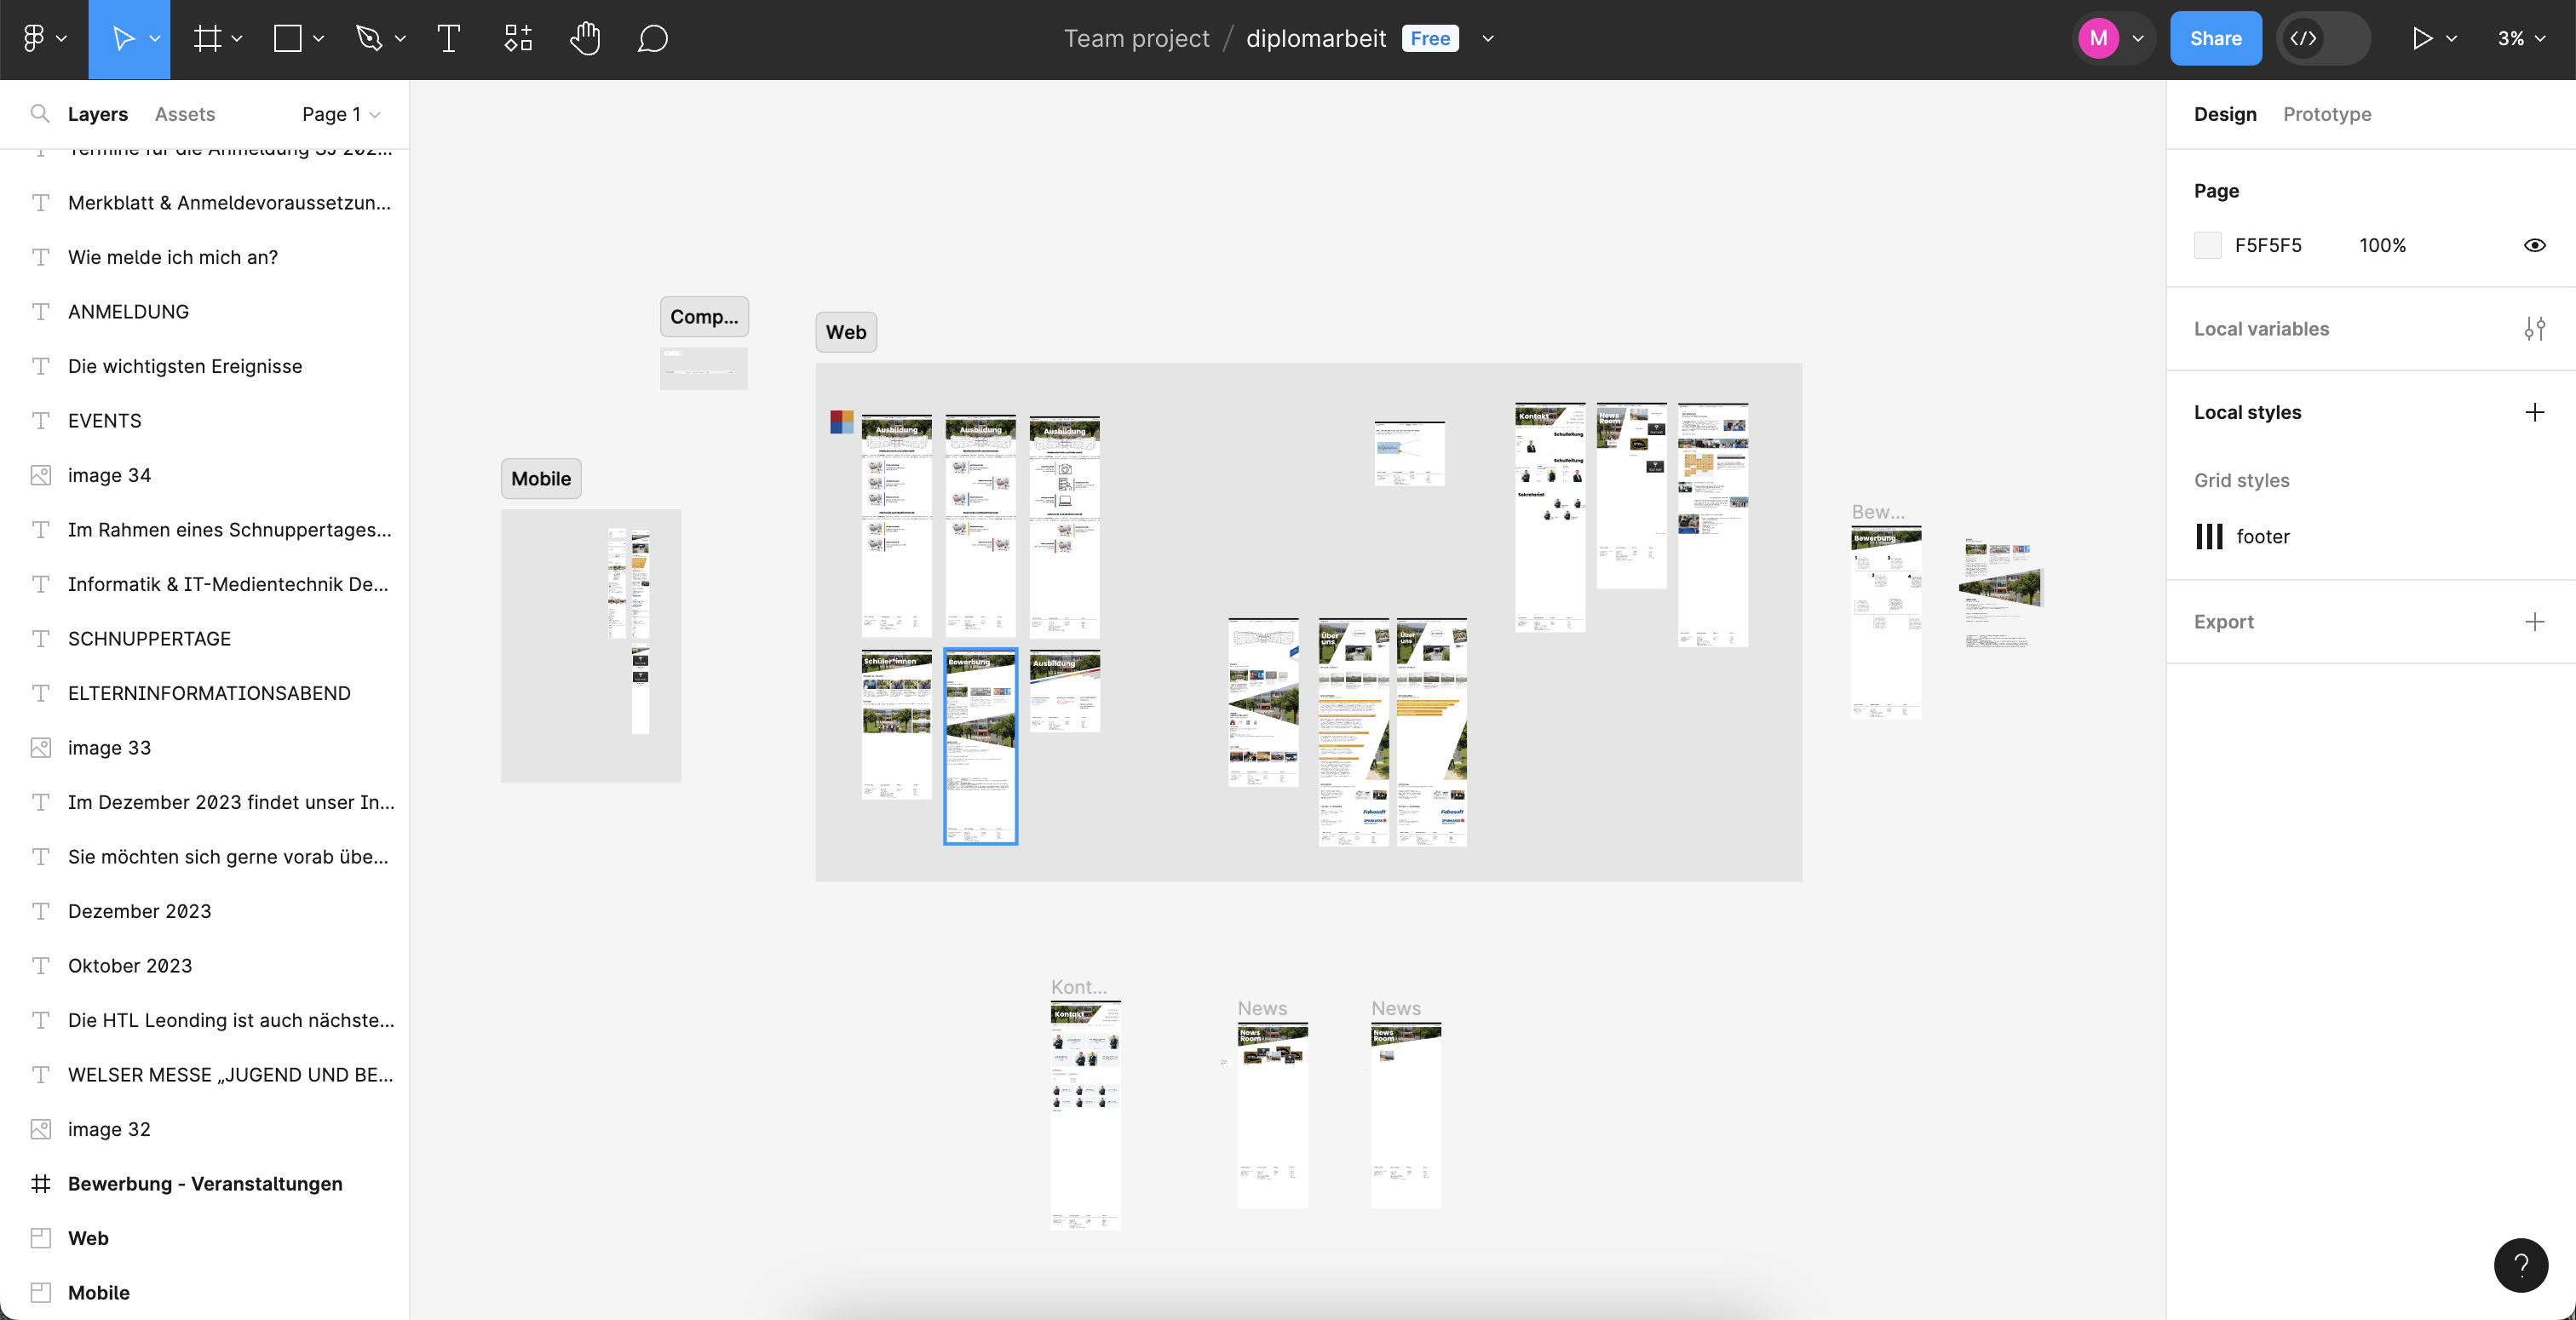
\includegraphics[width=\linewidth]{pics/figma.png}
      \caption{Entwurf mit Figma}
      \label{fig:impl:figma_entwurf}
   \end{minipage}
   \hspace{.05\linewidth}
\end{figure}

\section{Finales Design}
\setauthor{Angerer Mona}
Nachdem der Prozess des Usability-Testings und der Überarbeitungen einige Male durchlaufen
wird, entsteht am Ende ein optimiertes und finales Design. 

Dieses beinhaltet folgende Designelemente und unterscheidet sich in diesen Punkten zu der Gestaltung der bisherigen HTL-Website:


\subsection{Menu und Inhalt}
\setauthor{Angerer Mona}
   Im Vergleich zum alten Menu-Header (Siehe Abbildung \ref{fig:impl:header:alt}) hat der Neue (Siehe Abbildung \ref{fig:impl:header:neu}) statt 7 nur mehr 5 Elemente, um eine sauberere
   Ansicht zu schaffen und Verwirrung in der Navigation zu vermeiden. Die Inhalte aus dem Reiter \glqq News\grqq{} können nun durch einen Link auf der Seite
   \glqq Über uns\glqq{} erreicht werden, die Partnerfirmen stehen nun auf der Startseite. Der Menüpunkt \glqq Schüler:innen\grqq{} ist nun
   aum rechten Bildschirmrand platziert, um die Hauptelemente des Headers erneut zu vermindern und um eine Art \glqq Profil\grqq{}
   oder \glqq Einloggen\glqq{} zu suggestieren. Dort finden sich ebenfalls keine nur für bereits an der HTL Leonding
   lernende Personen, denn dieser Inhalt wurde umfassend in das LeoWiki ausgelagert. Stattdessen findet man unter 
   dem Reiter jetzt die an der Schule angebotenen Programme und SchülerInnenfotos, um einen persönlichen Einblick zu bieten und 
   den Wünschen und Vorschlägen der bei den Usability-Tests befragten Personen nachzugehen.

   \begin{figure}
      \centering
      
\includegraphics[scale=0.3]{pics/header_alt.png}
      \caption{alter Header}
      \label{fig:impl:header:alt}
  \end{figure}

  \begin{figure}
   \centering
   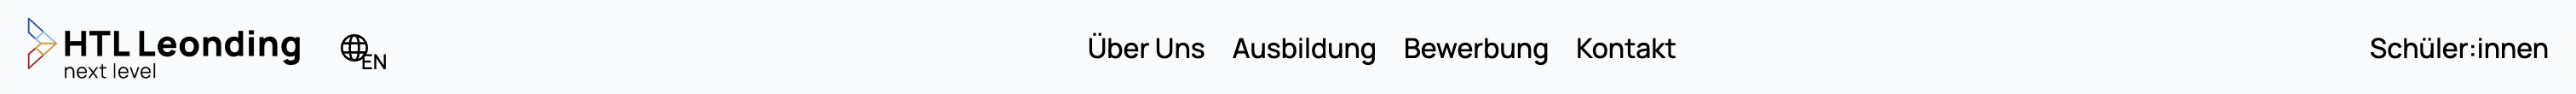
\includegraphics[scale=0.3]{pics/header_neu.png}
   \caption{neuer Header}
   \label{fig:impl:header:neu}
\end{figure}

\subsection{Farben und Formen}
\setauthor{Angerer Mona}
Da die bisherige Website sehr viele Farben beinhaltete, erschien sie überladen und überfordernd.
Nun wird bei der Gestaltung auf viel weiße Fläche gesetzt, die abgesehen von dem Bildmaterial lediglich von kleinen Akzenten 
in den vier Farben der Abteilungen, die auch im Logo vorkommen, und einer fünften Farbe, die eine Mischung der vier 
"HTL-Leonding-Farben" ist, unterbrochen wird. Der Trend zu viel "Whitespace" ist, wie im Kapiel \nameref{sec:Recherche} bereits
behandelt wurde, ein häufig aufkommendes, modernes Designkonzept.

Auch wurde statt auf das starre Block-Design auf mehr Abwechslung und Bewegung in den Formen gesetzt.
So ist das Dreieck eine der wichtigsten Elemente des neuen Webauftritts. Der Grund, weshalt die Wahl 
auf ausgerechnet diese Grundform gefallen ist, liegt in dem Logo der Schule. Dieses besteht aus einem Pfeil,
in dem sich die bereits angesprochenen vier Abteilungsfarben wiederspiegeln. Mittels der verschiedenen
implementierung des Dreiecks auf den unterschiedlichen Seiten der Website spiegeln sich so die Schrägen,
die man bereits im Logo findet, wieder. Auch erscheint der Gesamteindruck
dynamischer und spannender, was zu einer verbesserten User-Experience führt.

\subsection{Dynamik und Bewegung}
\setauthor{Angerer Mona}
Nicht nur die wiederholte Einbringung des nicht-typischen, wandelbaren Elements des Dreiecks
bringt mehr Spannung und dynamik in die Weboberfläche, auch sind viele sich bewegende Objekte auf 
der Website eingebunden. Um allerdings keine Unruhe und Stress in den Benutzern auszulösen, ist dieser
bewegte Content subtil und nicht zu oft angewendet und langsam in seiner Bewegung. Beispiele dafür finden sich 
auf der Seite "Abteilungen", wo sich eine Übersicht der Fächernamen von links nach rechts und umgekehrt
über den Bildschirm bewegt, oder auf den Seiten der einzelnen Abteilungen, wie Beispielsweise "Informatik - SSE", 
wo sich eine Reihe von Bildern, die die Fachrichtung beschreiben, sich vertikal über das Display bewegt.


\subsection{Animationen}
\setauthor{Angerer Mona}
Um das durch den vielen Whitespace erzeugte schlichte Design etwas aufzubrechen, wurde eine Strartanimation,
sowie Animationen für jede Abteilung eingefügt. Die Startanimation, die beim Aufrufen der Website 
abgespielt wird, beginnt mit dem HTL Leonding-Logo mit dem Schriftzug "HTL Leonding next level", geht dazu über dass 
der Schriftzug verschwindet, sich das Logo in die Mitte des Bildschrims bewegt und  in eine vereinfachte Graifk der HTL von oben verwandelt.
In der Schlussposition befindet sich die Grafik der HTL am rechten Bildschirmrand und die 
wichtigsten Events scrollen aus dem Gebäude. 
